\chapter{Project Planning}

This section aims to present the time organization as well as the cost management of the project. It is divided in two sections, the first one aims to present time line of the project, that is, how much time has been spent on each of the cycles present on Chapter 4. The second sections presents the cost planning.

\section{Temporal Planning}

On Chapter 4 we presented the six cycles necessary to realize the project. The time spent on each phase is variable depending on the difficulty of the tasks. The biggest amount of time spent goes to the Context Switch phase due to the difficulty of designing, implementing and debugging and all the concept involved in context switching. The phase dedicated to the  execution of a \textit{hello world}, serial output and command line interface shares a similar amount of time spent (around two months and a half) due to the extensive amount of research needed for the two first phases. Finally, the HDMI output phase and serial input phase were the shortest since they were pretty similar the phase 2 (i.e. serial output) and therefore, the amount of research were already done beforehand.

The project has officially started the 5th of October 2014 and finished the 25th of September 2015.

A Gantt diagram is displayed on figure \ref{fig:chapter7_gant_diagram} displaying graphically the time-lapse for each phase and process of each phase. 


\begin{figure}
\begin{center}
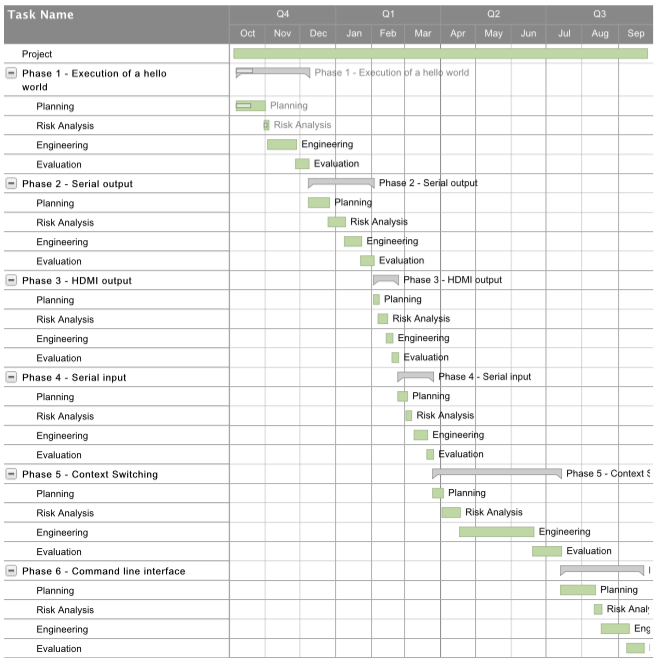
\includegraphics[width=1\textwidth]{includes/figures/chapter7_gant_diagram.png}  \\[0.5 cm]
\end{center}
\caption{Gant Chart of the Project}
\label{fig:chapter7_gant_diagram}
\end{figure}


\section{Cost Projection}

This section is aimed to perform an estimation of the physical resources needed and their related amount of money spent throughout the realization of the project. It is necessary to take into account the deprecation of the material being used. The project being realized in Spain, we will refer to the country's law dedicated the mater, that is the \textit{Ley del impuesto de sociedades}\cite{ley_impuesto_sobre_sociedades}. The amortization\cite{amortizacion_2015} of a computer is of \textit{8 years}. We will consider both the Raspberry Pi and the MacBook Pro to fall into that category.

As seen from the previous section, the project spans between eleven and twelve months, for our deprecation calculation we will therefore use a full year.

\begin{center}
\begin{table}[H]
    \centering
    \begin{tabular}{| p{2cm} | p{3.4cm} | p{3.4cm}| p{3.4cm} |}
    \hline
    \textbf{Material}        & \textbf{Cost for one unit}  & \textbf{Deprecation}& \textbf{Total for one year}\\\hline
    Personal computer       & \EUR{1500}                  & 8 years                     & \EUR{187,5} \\\hline
    Raspberry Pi B+         & \EUR{30}                    & 8 years                     & \EUR{3,75} \\\hline
    \multicolumn{3}{| p{8.8cm} |}{\textbf{Total}} & \textbf{\EUR{191,25}}\\ \hline
    \end{tabular}
    \caption{Cost projection for physical resources taking into account deprecation}
    \label{tbl:chapter7_cost_project_deprecation}
\end{table}
\end{center}



In terms of fungible resources, only electricity has been used. A MacBook Pro 13" uses about 12,1 Watts\cite{macbookpro_13_2013_energy_consumption}. A Raspberry Pi consumes about 1,21 Watts\cite{raspberry_pi_bplus_energy_consumption}. For a total of 13,31 Watts. Finally, the price per kWh is estimated to be \EUR{0,138280}\cite{tarifas_gas_luz}

We estimate the amount of average work of 17 hours a week with these devices, a total of 952 hours. We therefore can estimate the amount of energy spent to be \textit{12.67112kWh}. We can therefore estimate the amount of electricity spent to \textbf{\EUR{1,76}}.


Finally, we need to draw the cost of human resources. The amount of hour spent by each member can be obtained from the previous section. The table \ref{tbl:chapter7_human_resources_cost} shows the amount spent for each member.

\begin{center}
\begin{table}[H]
    \centering
    \begin{tabular}{| p{2cm} | p{3.4cm} | p{3.4cm}| p{3.4cm} |}
    \hline
    \textbf{Member}         & \textbf{Cost per hour} & \textbf{Hours worked}  & \textbf{Total}\\\hline
    Project Manager         & \EUR{35}             & 120 hours                & \EUR{4 200} \\\hline
    Requirement Engineer    & \EUR{20}             & 60 hours                & \EUR{1 200} \\\hline
    Analyst                 & \EUR{25}             & 80 hours                & \EUR{2 000} \\\hline
    Designer                & \EUR{25}             & 150 hours                & \EUR{3 750} \\\hline
    Developer               & \EUR{20}             & 210 hours                & \EUR{4 200} \\\hline
	Tester                  & \EUR{15}             & 110 hours                & \EUR{1 650} \\\hline
    \multicolumn{3}{| p{8.8cm} |}{\textbf{Total}} & \textbf{\EUR{17 000}}\\ \hline
    \end{tabular}
    \caption{Human resource cost}
    \label{tbl:chapter7_human_resources_cost}
\end{table}
\end{center}


With all these data, we can obtain the final cost of the project:


\begin{center}
\begin{table}[H]
    \centering
    \begin{tabular}{| c | c |}
    \hline
    \textbf{Concept}   & \textbf{Cost} \\ \hline
    Physical Resources	& \EUR{191,25} \\ \hline
	Fungible Resources & \EUR{1,76} \\ \hline
    Human Resources    & \EUR{17 000} \\ \hline
    Risk (15\%)        & \EUR{2 578,96} \\ \hline
    \textbf{Total without Tax}     & \textbf{\EUR{19 771,97}}\\ \hline
    Taxes 				& \EUR{3 954,394} \\ \hline
    \textbf{Total with Tax} & \textbf{\EUR{23 726,364}} \\ \hline
    \end{tabular}
    \caption{Cost Projection Total}
    \label{tbl:chapter7_total_cost_projection}
\end{table}
\end{center}

